\begin{figure}[H]
  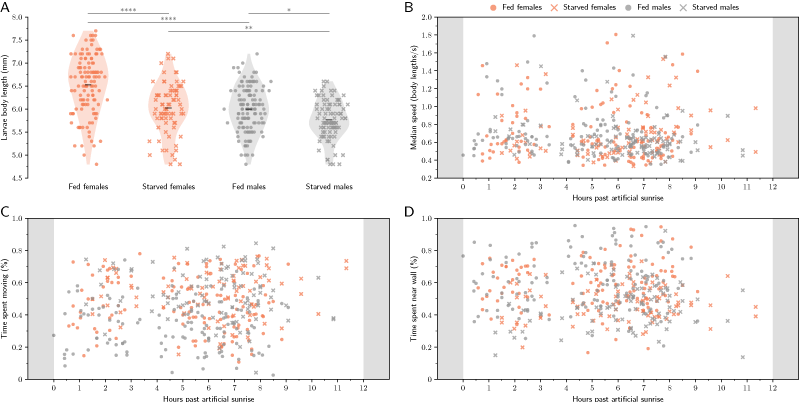
\includegraphics[width=\linewidth]{Figures/images/S1.eps}
  \caption{\textbf{Effects of sex, physiological state, and circadian timing on larval physiology.} A-D: Fed females (orange dots, n=120) and males (grey dots, n=128), starved females (orange X markers, n=79) and males (grey X markers, n=89). A: Violin plot. Scatter points show the body length (mm) for each individual, and the black bar is the mean across all individuals; asterisks denote significance values (Welch's t-test). Larval body length is influenced by sex and starvation state. B: No change was observed in median speed (body lengths/s). Note that the sampling rate throughout the day was not consistent due to the work schedule of experimenters involved in the project. C: No change was observed in time spent moving throughout daylight hours. D: No change was observed in proportion of time spent within one body length of the wall throughout daylight hours.
}
\end{figure}

\null
\vfill